\documentclass[12pt]{article} 
\usepackage[legalpaper, portrait, margin=.5in]{geometry} 
	\geometry {
		top=.5in,
		bottom=1in
	}
\usepackage[utf8]{inputenc} 
\usepackage{verbatim} 
\usepackage{graphicx} 
\usepackage{scrextend}

\title {Machine Learning Notes}
\author {DS210}

\begin{document}
	\newpage \vfill
	\centering \textbf{Machine Learning Notes}
	\begin{itemize} %begin bullet points 
		\item fundamentally a taste of classification, where you identify the category of a new piece of data based upon some training data that was previously publised 
		\begin{enumerate} % begin numbers 
			\item given data from a training set (60\%), we develop a model which we use to predict the results of new data we don't have yet
			\item apply the model from 1 to a verification set (20\%) (the test set), where we text the accuracy of our prediction. We know the answer for the verification set, but we do not train on them \thanks steps 1 and 2 occur in a cycle 
			\item apply the model to the test set (20\%), which is hidden/secret/safe from developers		
		\end{enumerate}
		\item success: if you were to be given an answer, your model would match the answer 
		\item models that are bad: 
		\begin{itemize} % first indented bullets 
			\item memorizing the verification set 
			\begin{figure}[h] 
				\centering
				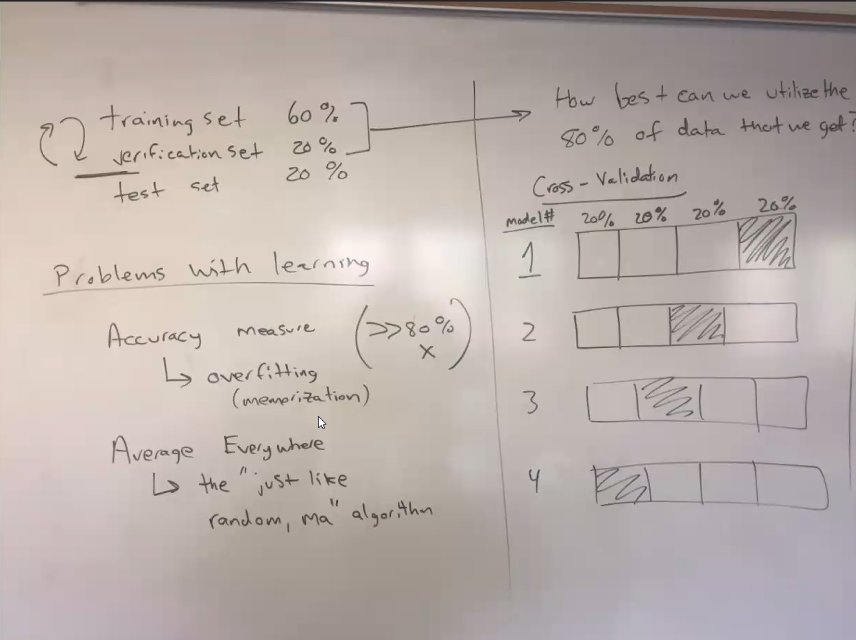
\includegraphics[scale=0.5]{diagram1.png} 
			\end{figure}
			\begin{itemize} % second indented bullets 
				\item this may happen by accident if we have access to all of the data
				\item this is why some of the data should be hidden to the developer (the actual test set, not the DS110 set)
			\end{itemize}
			\item how best can we utalize the 80\% of data that we got? 
			\begin{itemize} % second indented bullets, again
				\item you can run these results through a second classifier 
				\item dave really likes neural networks 
				\begin{figure}[ht] 
					\centering
					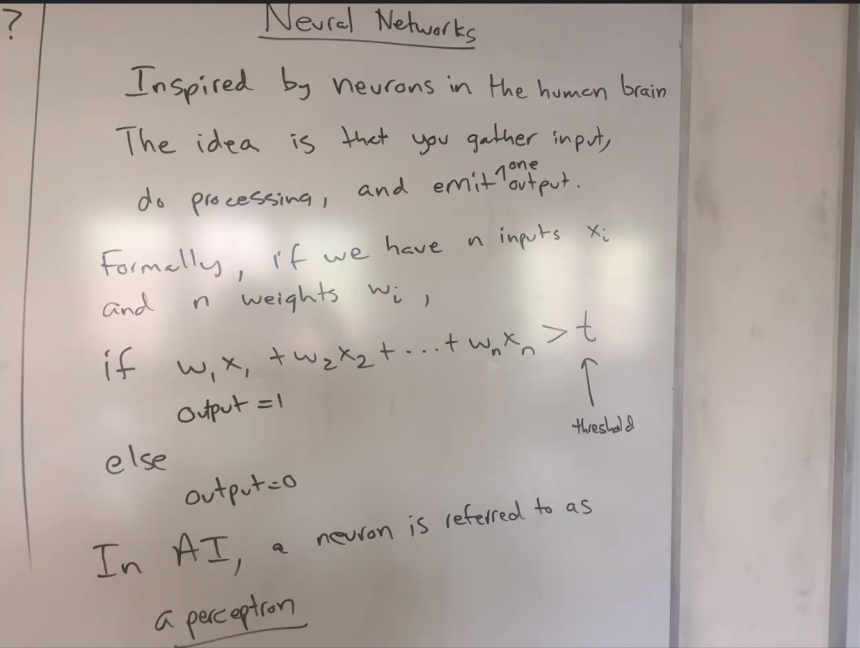
\includegraphics[scale=0.5]{neuralnetworks.png} 
				\end{figure}
				\item decisions trees are also a thing 
				\begin{itemize} % third level indented bullets 
					\item basically think of 20 questions, we did an inclass example with the titanic dataset 
				\end{itemize}
			\end{itemize}      
		\end{itemize}
	\end{itemize}
	\vfill
	\clearpage

	\newpage \vfill
	\textbf{\centering Decision Tree Learning}
	\begin{itemize}
		\item you have some sort of splitting attribute, in this example: sex, age, pclass, survived 
		\item you then follow the tree that based on the criteria you are givens
		
		{\centering 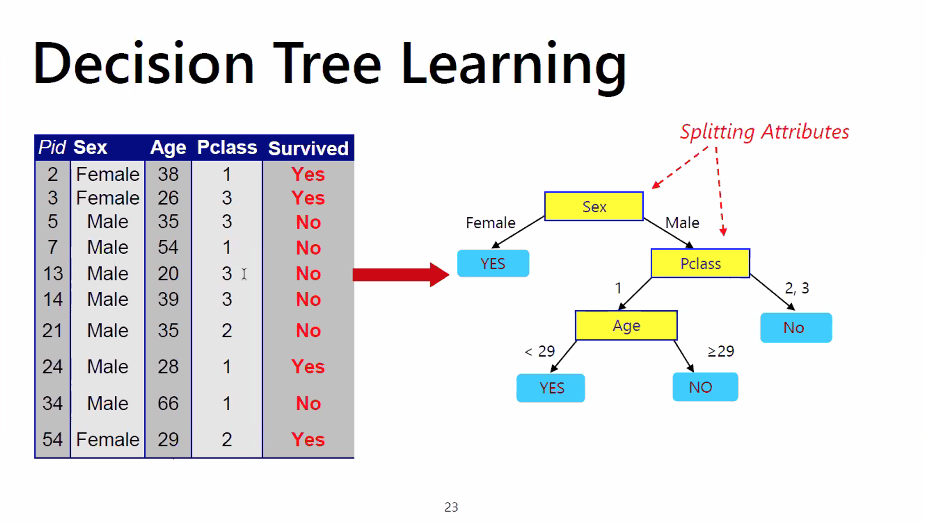
\includegraphics [scale=.5] {decisiontree.png} 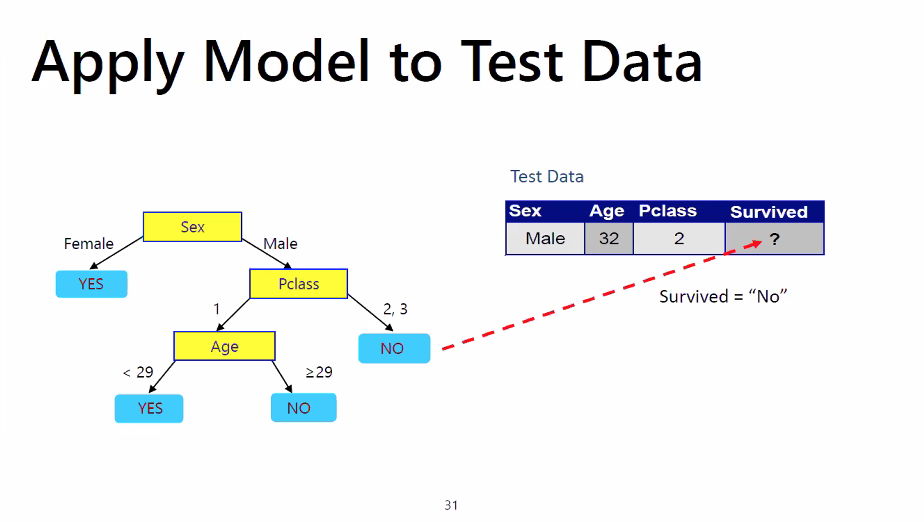
\includegraphics[scale=.5]{appliedmodel.png}
		\item it is important to note that the order of splitting factors matters, but sometimes they may produce the same results}
		\item How do we get a tree? 
			\begin{itemize}
				\item exponentially many decision trees are possible 
				\item finding the optimal tree is infeasible
				\item greedy methods find that near-optimal solutions do exist 
				\begin{itemize}
					\item greedy methods provide common sense solutions (i.e. travel south to go from butler to downtown)
					\item could also not be optimal (i.e. cross a river going east to west by going south instead of traveling west to the bridge and then crossing)
				\end{itemize}
			\end{itemize}
		\item Tree Induction
			\begin{itemize}
				\item Greedy strategy 
				\begin{itemize}
					\item split based on attribute test that optimizes a criterion
				\end{itemize}
				\item issues
				\begin{itemize}
					\item how to split the records 
					\begin{itemize}
						\item what attribute test condition? 
						\item how to determine the best split?
						\item when do we stop?
					\end{itemize}
					\item attribute types 
					\begin{itemize}
						\item nominal
						\item ordinal
						\item continuous 
					\end{itemize}
					\item order of split 
					\begin{itemize}
						\item 2-way split
						\item multi-way split 
					\end{itemize}	
				\end{itemize}
			\end{itemize}
		\item example 

			{\centering 
			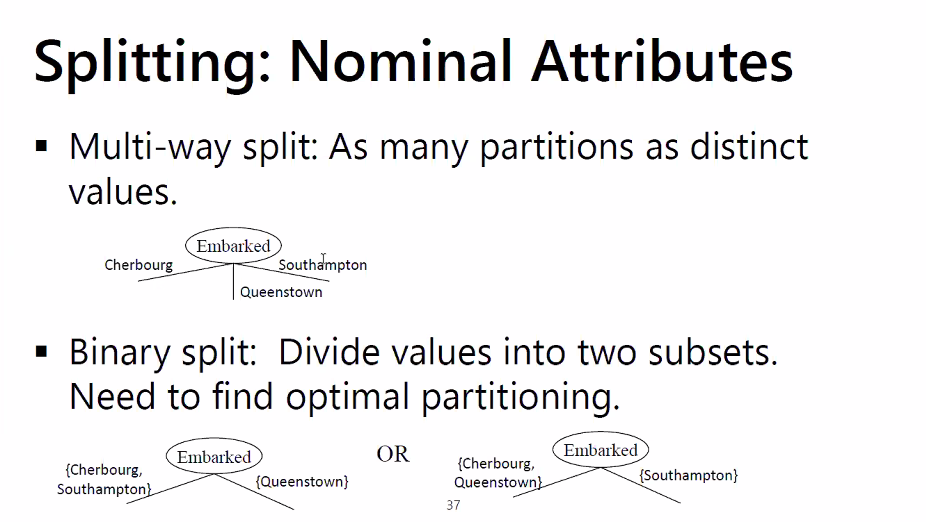
\includegraphics[width=2.25in]{splitnom.png}
			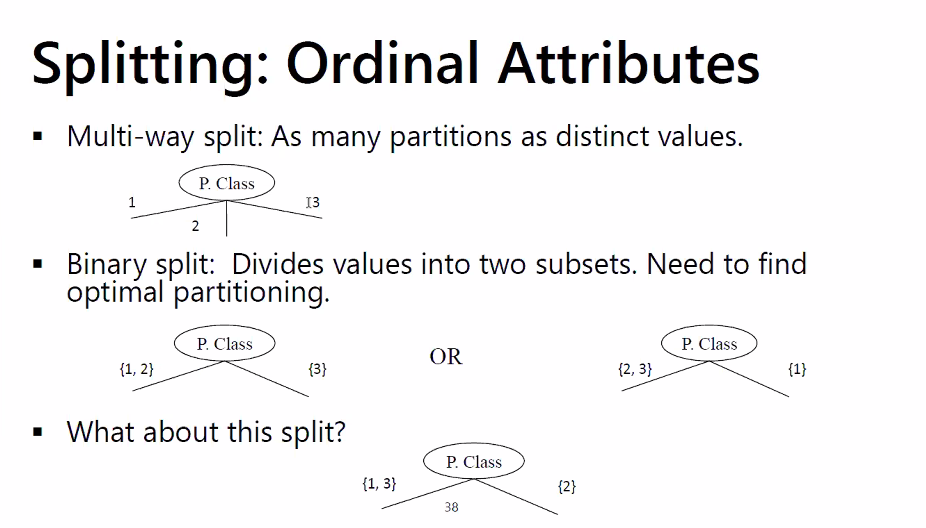
\includegraphics[width=2.25in]{splitord.png}
			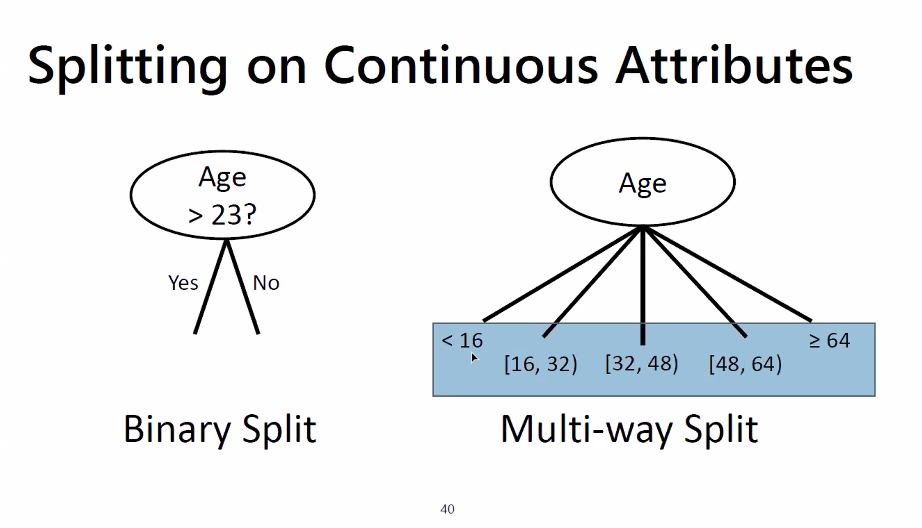
\includegraphics[width=2.25in]{splitcontinuous.png}
			\newline \newline
			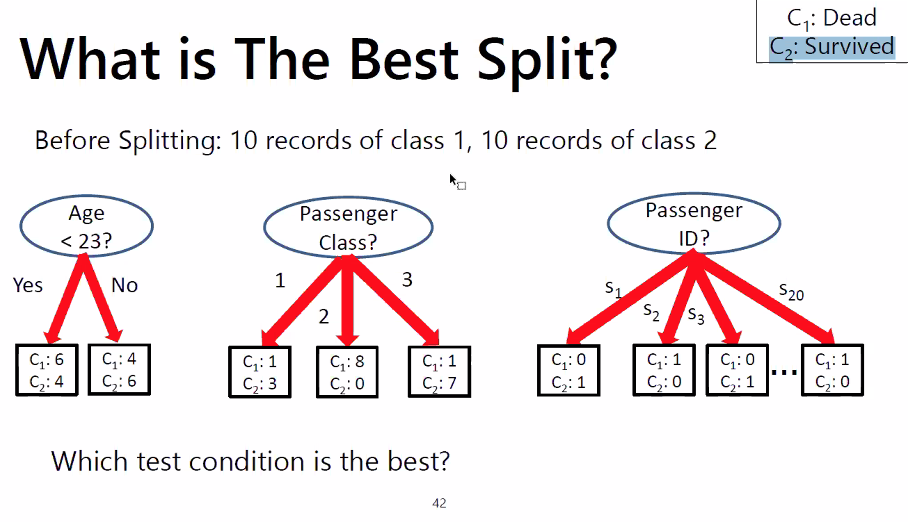
\includegraphics[scale=.45]{bestsplit.png}}
			
		\item you want the split to be heavily skewed, so that you don't necessarily have to ask another question to have a good guess
		\item greedy approach 
		\begin{itemize}
			\item homogeneous class distribution preferred 
		\end{itemize}
		\item need a measure of node impurity - aka a way to define what an impure node is 
		\item use node impurity to determine what nodes to start with 
		\item start with the most pure nodes possible 
		\item things you may want to specify:
		\begin{itemize}
			\item the height and the width. If you make it too wide then you did not skew nodes well enough... if you make it too tall you have made too many decisions before you predict
			\item you also may want to limit the branching factor 
			\item the smallest number of items in a category (node density)
			\item how to do splits
			\item GINI/entropy
		\end{itemize}
		\item decision trees are just one gigantic if statement 
		\item PROS 
		\begin{itemize}
			\item intuitive: easy interpretation for small trees 
			\item non parametric: incorportates both numeric and categorical attributes
			\item fast: once rules are developed, prediction is rapid
			\item robust to outliers: won't affect the majority classification
		\end{itemize}
		\item CONS
		\begin{itemize}
			\item overfitting: must be trained with great care, must put limits so that it does not overgrow --- must prune the tree 
			\item rectangular classification: recursive partitioning of data may not capture complex relationships
			\item hard to reconsider kinds of relationships -- sometimes your classification may need to stretch across your partition lines
		\begin{itemize} \item Example: age may not always do the same thing, so you either have to ask again about it later, or it doesn't do a good job of explaining \end{itemize}
		\end{itemize}
	\end{itemize}
	\vfill
	\clearpage




	\newpage \vfill
	\textbf{\centering Measures of Node Impurity}
	\begin{itemize}	
		\item GINI Index \newline
			{\centering 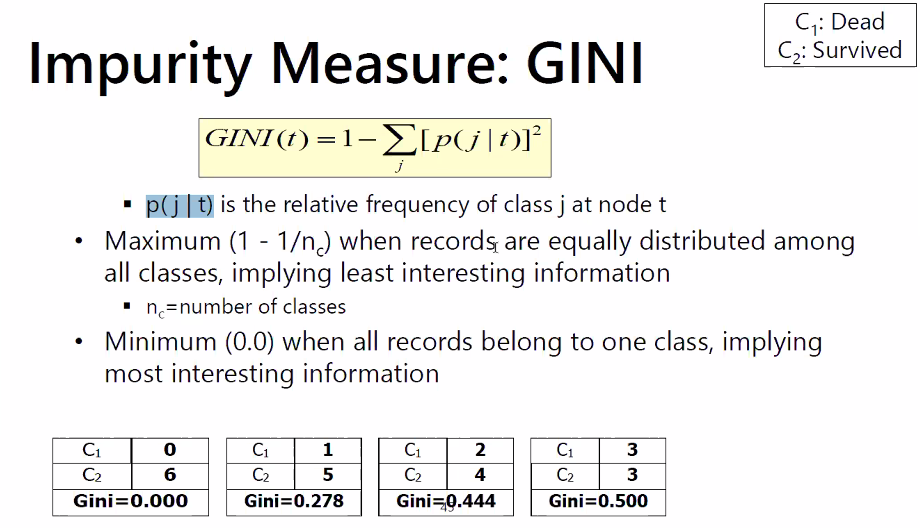
\includegraphics[scale=.5]{gini.png}}
			{\centering 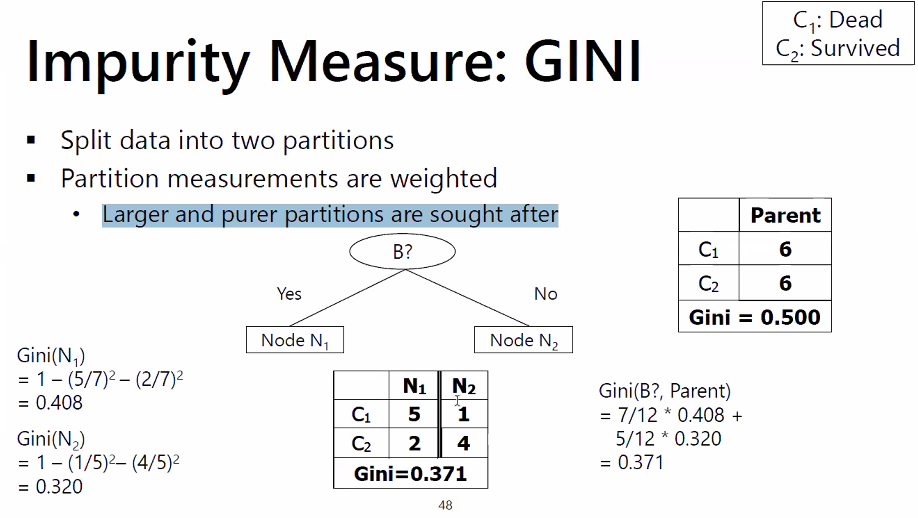
\includegraphics[scale=.5]{impurity.png}}
			\newline
			\begin{itemize}
				\item perform this calculation for every candidate B until you determine the best B to use for the first node in the tree 
				\newline
			\end{itemize} 
		\item Entropy
		\begin{itemize}
				\item measures the amount of chaos in the decision and also what the information that it encloses 
				\item highly uncategorizable data works well with this 
				\item less sensitive to overfitting
				\item slightly more obtuse, i.e. it isnt as clear why it classifies the way it does 
		\end{itemize}
		{\centering 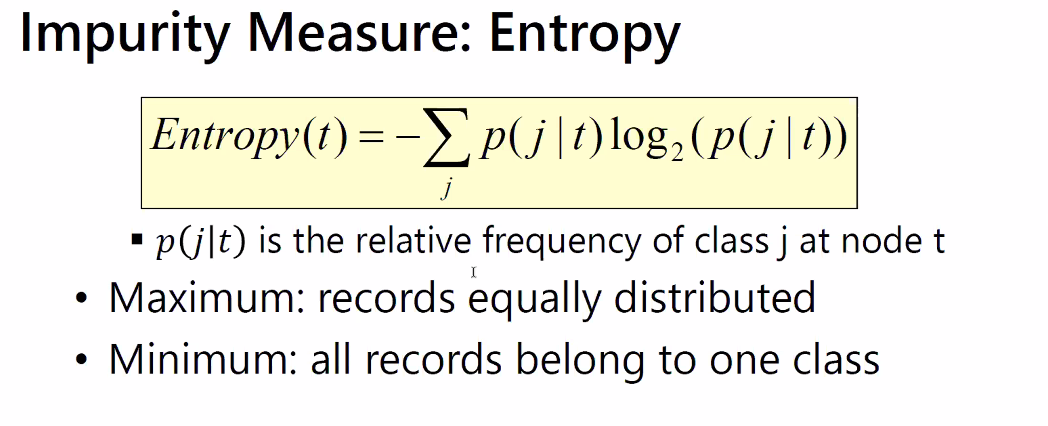
\includegraphics[scale=.5]{entropy.png}}
		\item Misclassification error \newline \newline
		{\centering 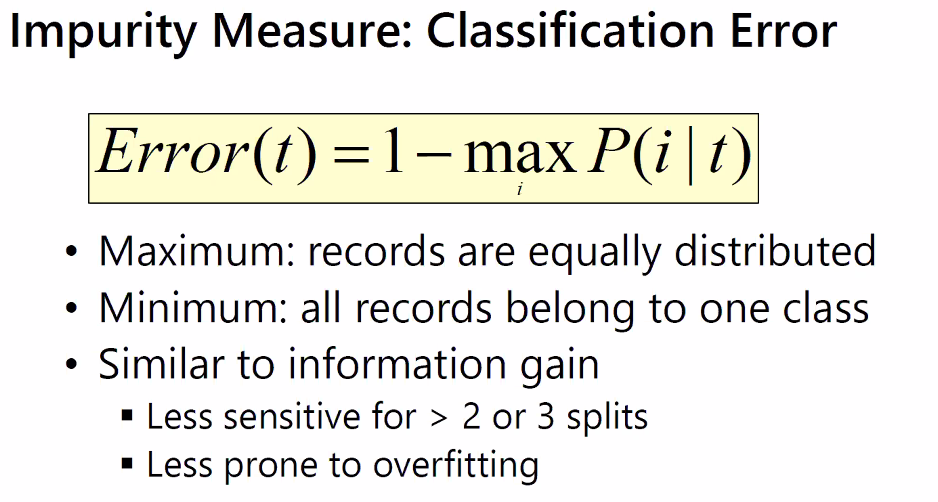
\includegraphics[scale=.5]{classification.png}}
	\end{itemize}
	\vfill
	\clearpage




	\newpage \vfill
	\textbf{\centering Ensemble Methods, Random Forests, and Boosting}
	\begin{itemize}
		\item \textbf{Ensemble Methods}
		\begin{itemize}
			\item improve model performance by combining \textit {independent} multiple models
			\item basic idea: monopolized on the monty carlo effect, if you're rolling the die of classification, the chance that all dies fail at the same time is really low
			\item can be used for both classification and regression \newline
			{\centering 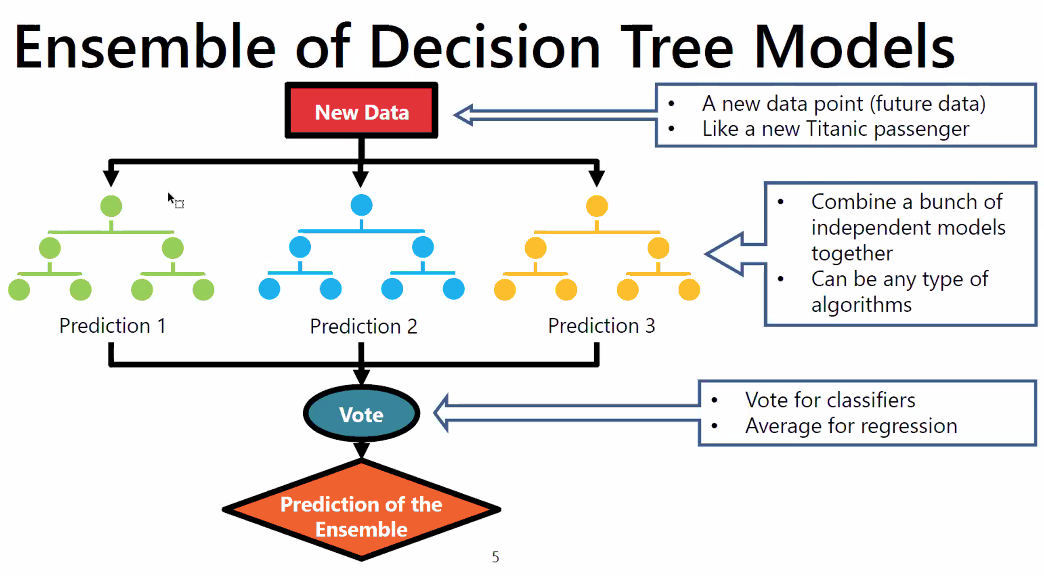
\includegraphics[scale=.5]{ensemble.png}}
			\item why does it work?
			\begin{itemize}
				\item suppose there are 25 base classifiers 
				\begin{itemize}
					\item each classifier has error rate = 0.35
					\item assume classifiers are independent 
					\item probability that the ensemble classifer makes a wrong prediction: \newline
					{\centering 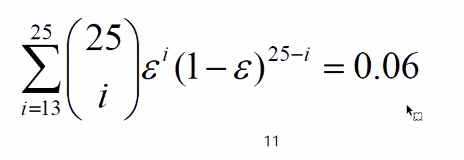
\includegraphics[scale=.5]{prediction.png}}
				\end{itemize}
			\end{itemize}
			\item two major methods:
			\begin{itemize}
				\item bagging (all classifiers are created equal) -- you bag until you get the same number as the original sample
				\begin{itemize}
					\item reduces variance in estimate because you're constantly changing the sample that you're working with
					\item prevents overfitting, because you cant have any guarentee that a specific piece of data may be in a given dataset 
					\item robust to outliers because they will, most likely, in general, be less likely to be selected than other stuff 
				\end{itemize}
				{\centering 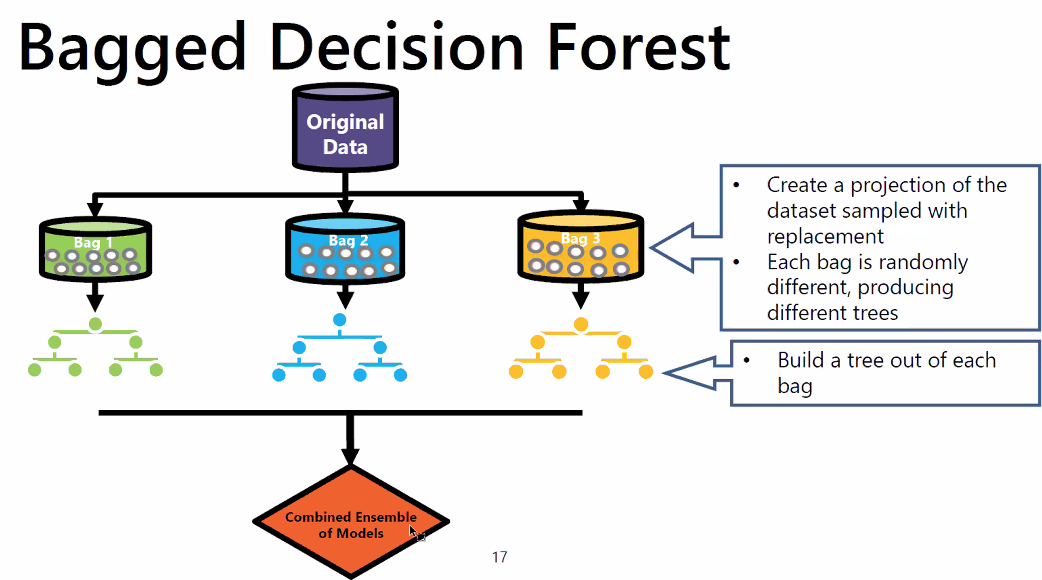
\includegraphics[scale=.4]{bagging.png}}
				{\centering 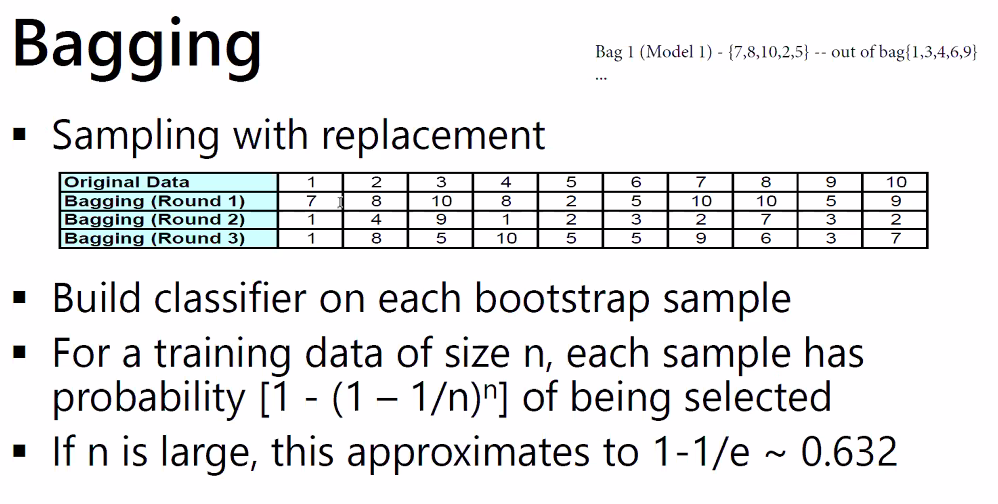
\includegraphics[scale=.4]{bagging1.png}}
			\end{itemize}
		\end{itemize} 
		\item \textbf{Random Forests} 
			\begin{itemize}
				\item an ensemble classifier using many decision tree models
				\item can be used for classification or regression 
				\item two key ingredients needed:
				\begin{enumerate}
					\item bagging (or sampling the data)
					\item random subset of features (or columns) when splitting nodes within trees -- we say (randomly) what you're allowed to split on 
				\end{enumerate}
				\item it is important to note that a less correlation also produces a weaker model
			\end{itemize}
			\newpage
			{\centering 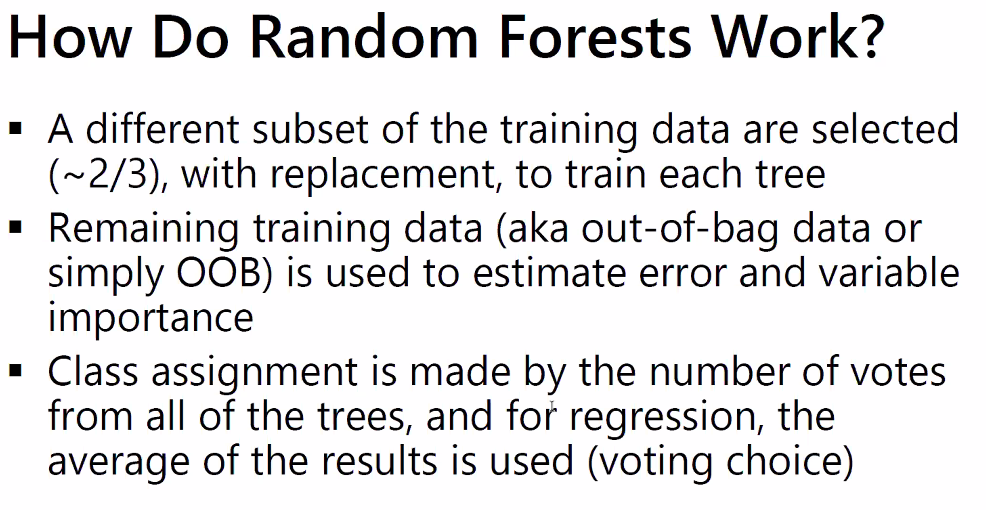
\includegraphics[scale=.45]{forest.png}}
			{\centering 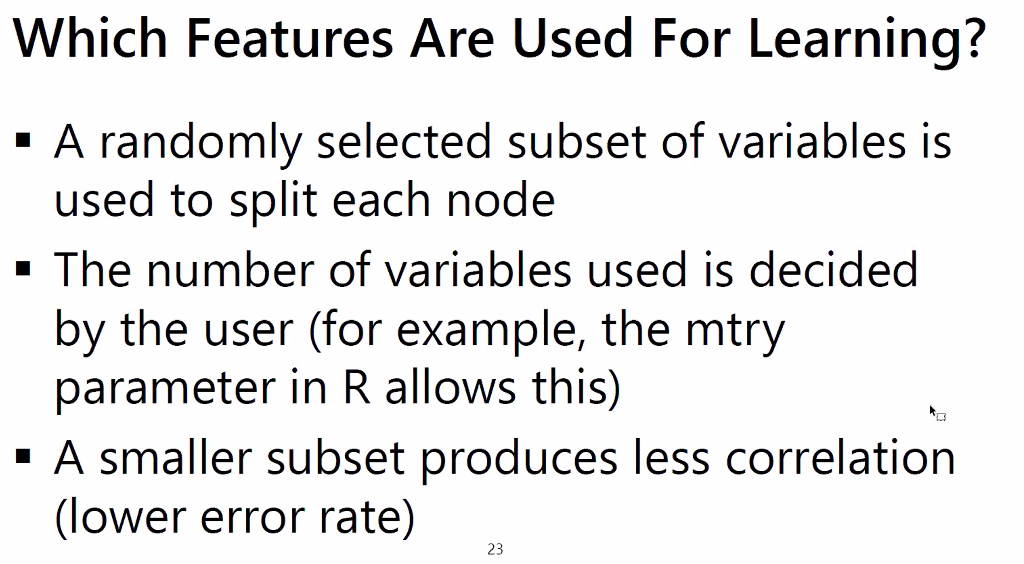
\includegraphics[scale=.45]{choices.png}\newline}
			{\centering 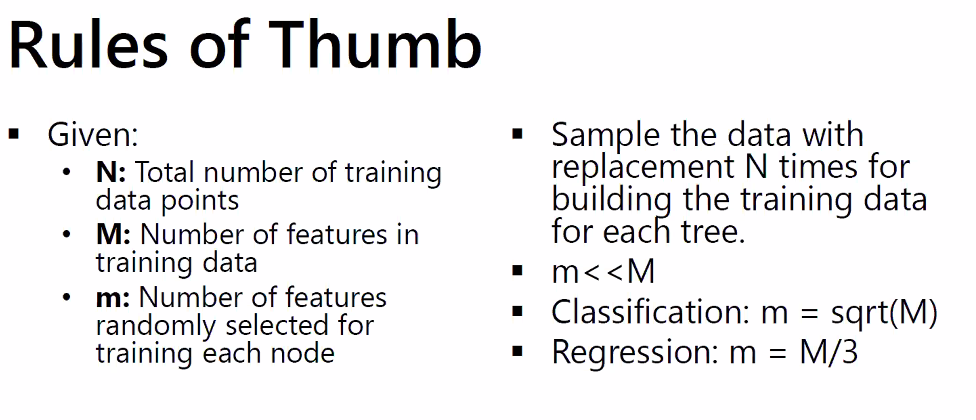
\includegraphics[scale=.45]{rules.png}}
			{\centering 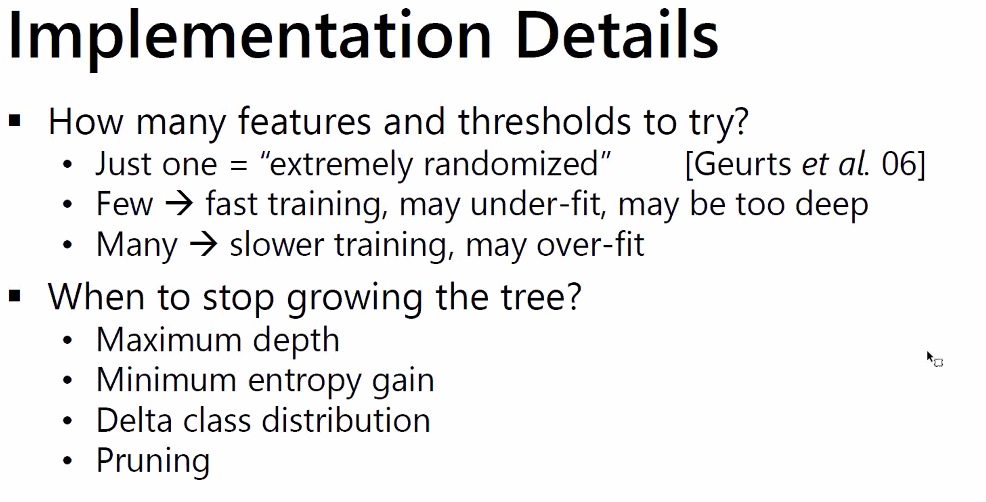
\includegraphics[scale=.45]{implementation.png}}
		\item \textbf{Boosting}
		\begin{itemize}
			\item an iterative procedure to adaptively change distribution of training data by focusing more on previously misclassified records
			\begin{itemize}
				\item initially, all N records are assigned equal weights
				\item then, when you get stuff wrong, you increase the weights of that stuff 
				\item do these things recursively ^^
			\end{itemize}
			{\centering 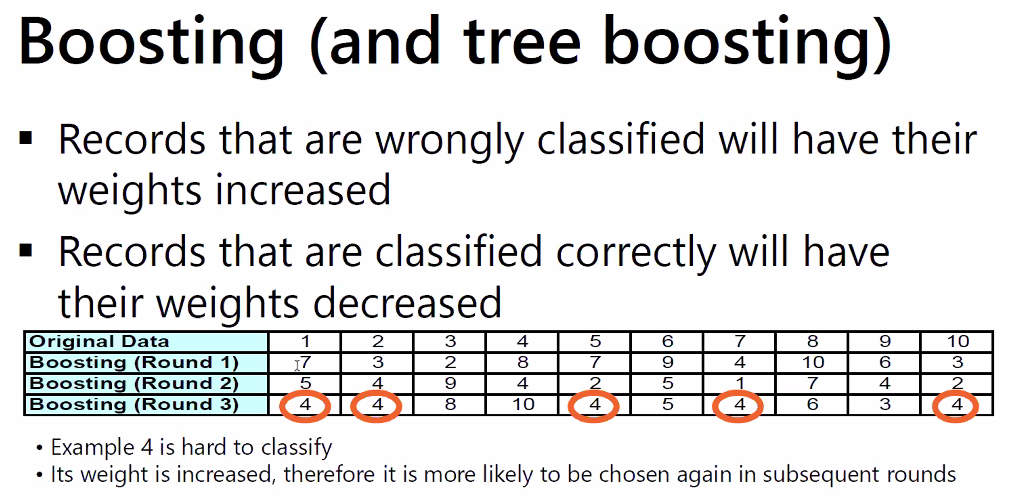
\includegraphics[scale=.45]{boosting.png}}
			\item boosting intuition
			\begin{itemize}
				\item we adaptively weight each data case 
				\item data cases which are wrongly classified get high weight (the algorithm will focus on them)
				\item each boosting round learns a new (simple) classifier on the weighed dataset
				\item these classifiers are weighed to combine them into a single powerful classifier
				\item classifiers that obtain low training error rate have high weight 
				\item we stop by monitroing a hold out set 
			\end{itemize}
			{\centering 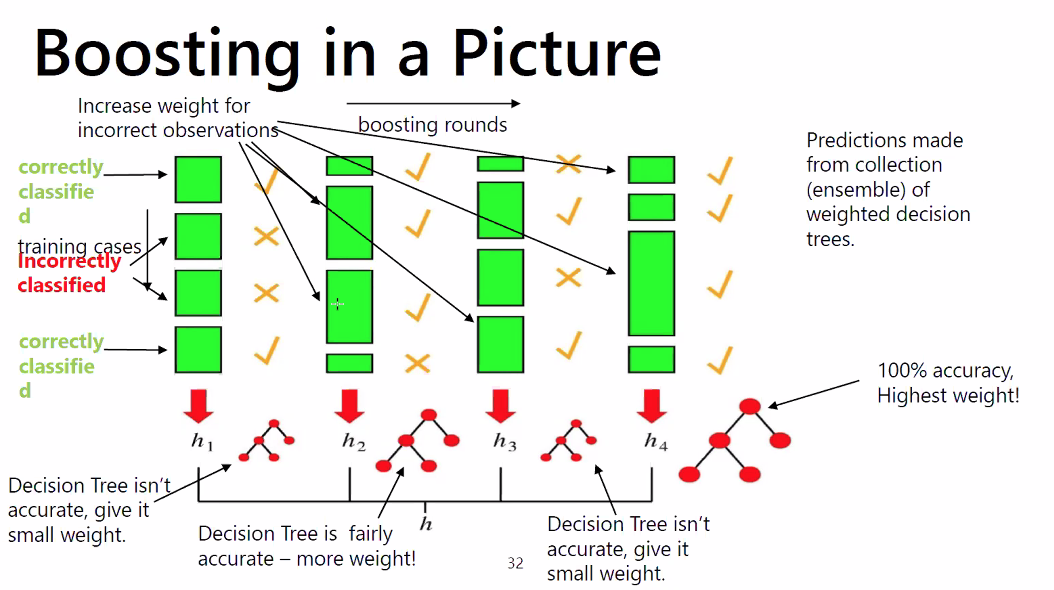
\includegraphics[scale=.45]{boostexample.png}}
			\item adaboost \newline
			{\centering 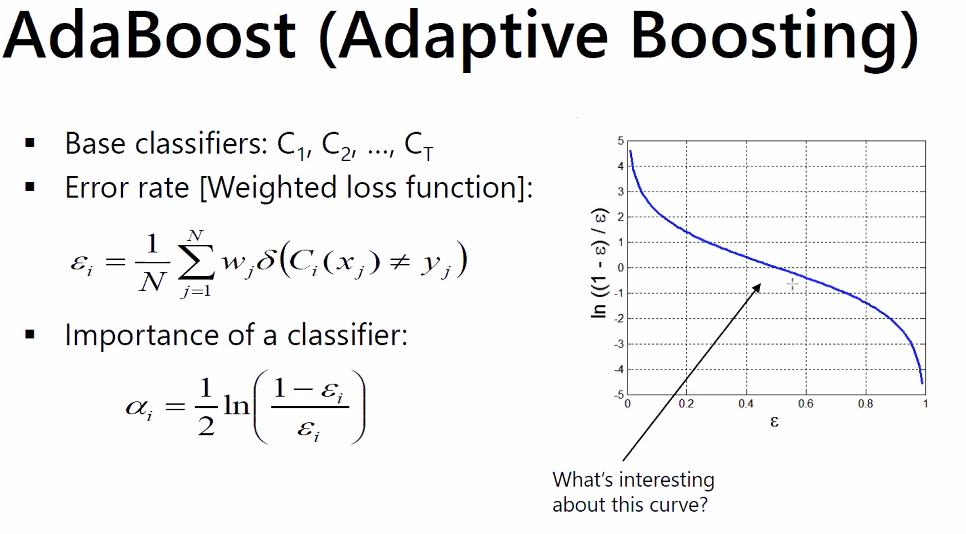
\includegraphics[scale=.45]{adaboost.png}}
			\item common misconception: a random forest and a boosted decision tree are \emph{not} the same 
		\end{itemize}
	\end{itemize}
	\clearpage


	\newpage \vfill
	\textbf{\centering Neural Networks}
	\begin{itemize}
		\item Perceptrons
		\begin{itemize}
			\item inspired by neurons in the human brain 
			\item basic idea: gather input, do some processing, and emit \emph{one} output
			\item formally, if we have n inputs $x_i$ and n weights $w_i$, 
			if $w_1x_1 + w_2x_2 + ... + w_nx_n > t$ where t is a given threshold, then output 1
			else output 0 
			\item t, the threshold will be some value between 0 and 1
			\item this whole thing is called a neuron/perception. In AI, a neuron is called a perceptron
			\item each item has its own node, with certain weights on their path to the perceptron to determine one output 
			\item starting weights are given randomnly and then redetermined each time the model is run and something goes wrong
			\item incremental gradient: the step size, in which we shall make modifications to the beginning weights 
			\begin{itemize}
				\item correction factor for wrong answers from the perceptron 
				\item we only adjust the things that contribute to us being wrong, in the student example, its the things with a value of 1
				\item if we predicted too high, we decriment, if too low, we increment
			\end{itemize}
			\item what the fuck do you do if you can't converge? 
			\item CRITICAL FLAW: very simple functions that they cannot predict 
			\begin{itemize}
				\item cannot predict exclusive or correctly (LOL FAIL)
			\end{itemize}
			\item the lower t, the faster it trains, and the more likely it is to be wrong 
			\item this leads to "iterative deepening" in terms of training
			\item in reality, the step size is discounted over time, i.e. it is not fixed 
		\end{itemize}
		\item A Generalized Neural Network 
		\begin{itemize}
			\item typically, you'll have a bipartide connected graph as your network 
			\item there is a 'hidden' layer of perceptrons in the middle 
			\item typically, you'll get multiple outputs at a time
			\item to solve general problems on this neural network is... 
			\begin{itemize}
				\item perceptions now emit a real number [0,1]
				\item these real numbers \emph{propogate an error} and cause a problem 
				\item a technique called back propogation allows you to recompute based on future results to limit the effect of this error 
			\end{itemize}
		\end{itemize}
	\end{itemize}
	\clearpage


	\newpage \vfill
	\textbf{\centering Genetic Algorithms}
	\begin{itemize}
		\item the basic idea is that you have some number of possible solutions called genomes. Then, we will "breed" (and possibly mutate) these genomes to create \emph{offspring}. All offspring are scores using some scoring function, and the most promising ones become part of an updated genome set 
		\item Examples: 
		\begin{itemize}
			\item Y\#N\# --> if I was top 10 last year, and I did not work hard, I will be top 10 this year 
			\item N\#YN --> I did not get top ten last year, and I did work hard, and I did not drink --> top 10 this year
		\end{itemize}
		\item Scoring function: test the rule for correctness on the table and represent it with a probablity of predictive success (for example, accuracy)
		\item Breeding: Y\#N\# and N\#YN -- arbitarily divide in half, then flop to create Y\#YN and N\#N\#
		\item Mutation: Y\#N\# and N\#YN and Y\#YN and N\#N\# --> N\#NY 
		\begin{itemize}
			\item lots of math goes into this, including concepts called simulated armealing and hill climbing (gradient descent)
		\end{itemize}
		\item Example:
		\begin{itemize}
			\item S = {\#Y\#\# (2/6 probability), N\#YN (3/6), YY\#\# (4/6), \#YY\# (4/6), \#\#\#N (4/6)}
			\item you basically just pick two of them, and glue them together (breeding)
			\item YY\#\# and \#YY\# become YYY\# and \#Y\#\# 
			\item do the following over and over again until stable 
			\begin{enumerate}
				\item breed
				\item mutate
				\item purge bad genomes from the genome set 
			\end{enumerate}  
		\end{itemize}
	\end{itemize}


\end{document} 